The reference data for congestion measurement is provided by ASTRA (Bundesamt für Strassen). There are four datasets: 
\begin{itemize}
\item Dataset 1: measurement of 2014 July, 18. - 19.
\item Dataset 2: measurement of 2014 August, first
\item Dataset 3: measurement of 2014 July, 25. - 26.
\item Dataset 4: measurement of 2014 August, second
\end{itemize}

In a first step the model will be trained by dataset 1 and 2. The authors wrote a program which calculates specified values of a specified variable (moveProb and moveCorr) for a given number of times. With other words, it finds the optimal parameter values that minimize the error of measured congestion. In a second step, the datasets 3 and 4 are used to evaluate the previous trained model.

\subsection{Preparing dataset -- curve fitting}
The timestamps for the measurement are irregular. In order to compare the congestion from the model to the reference data, the breakpoints will be interpolated. The resulting curve can be used to generate regular timestamps for measurement. The authors have opted for a linear interpolation. That means that every point will be connected by a straight line with its neighbour, see on the figures below. A linear interpolation is reasonable because the congestion length between two breakpoints cannot change very quickly.

%Die Referenzdaten vom ASTRA (Bundesamt für Strassen) enthalten Staumessungen. Diese sind in unregelmässigen Abständen gemessen. Um einen Vergleich mit der Messung im Modell 
%vorzunehmen, werden die Datenpunkte Interpoliert. Die gefundene Kurve wird dann benutzt, um regelmässige Messungen zu generieren. Die Authoren haben sich für eine lineare %Interpolation entschieden, sodass Punkt zu Punkt mit einer Geraden verbunden wird. Dies ist sinnvoll, weil die Länge des Staus zwischen zwei Punkten nur geringfügig ändern kann.

\begin{figure}[H]\centering
\includegraphics[width=.9\textwidth]{dataset1.pdf}
\caption{Dataset 1}
\end{figure}
\vspace*{-1.5cm}
\begin{figure}[H]\centering
\includegraphics[width=.9\textwidth]{dataset2.pdf}
\caption{Dataset 2, added regular measurements for comparison}
\end{figure}

\subsection{Train model}
There are two parameters to fit the model:
\begin{itemize}
\item moveProb: describes how accurate cars moving forward
\item moveCorr: increases moveProb in case of congestion
\end{itemize}

The program optiFinder was written to find the best setting of these two parameters. Important here by are the quantities \textit{prediction} and \textit{precision}.
The latter describes the relative ratio between the area outside the intersection and the area of the reference data itself. One can imagine two portions $A$ and $B$ and its intersection $A \cap B$. The precision would be $\textrm{precision} = 1 - (A \cup B - A \cap B) / A$, where $A$ is the area from the reference data.

Prediction is the ratio between all x-values that are inscribed by the intersection of the two curves and the reference curve. The big difference to precision is the way of counting. It would be very beneficial for the prediction value, if there is a lot of congestion. The outcome of this would be a poor precision value. That's why precision and prediction are used to find the optimal parameter. Because precision is more important, the weight for it is three times greater than for prediction.

\begin{figure}[H]
\begin{minipage}[t]{.5\textwidth}
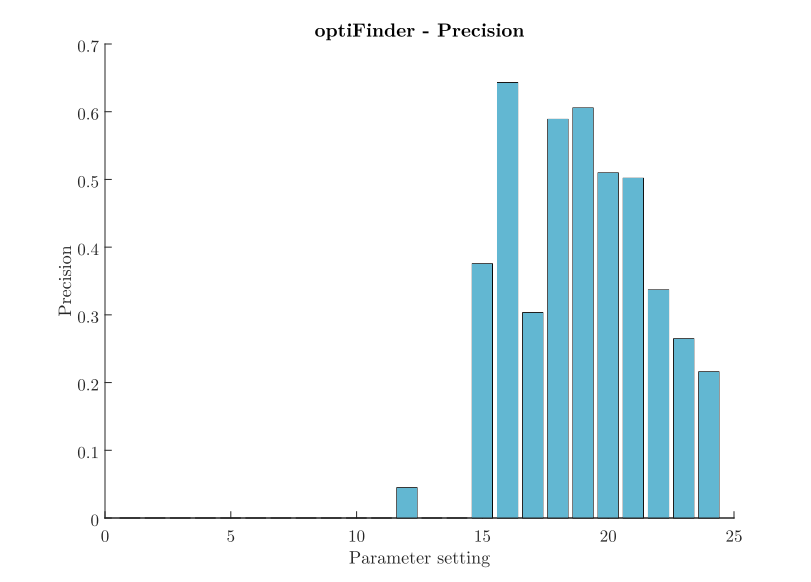
\includegraphics[width=\textwidth]{precision.pdf}
\end{minipage}
\begin{minipage}[t]{.5\textwidth}
\includegraphics[width=\textwidth]{prediction.pdf}
\end{minipage}
\caption{left: precision, right prediction for Dataset 2}
\end{figure}

The weighting of prediction and precision lead to the values for moveProb and moveCorr.


\begin{figure}[H]
\begin{minipage}[t]{.48\textwidth}
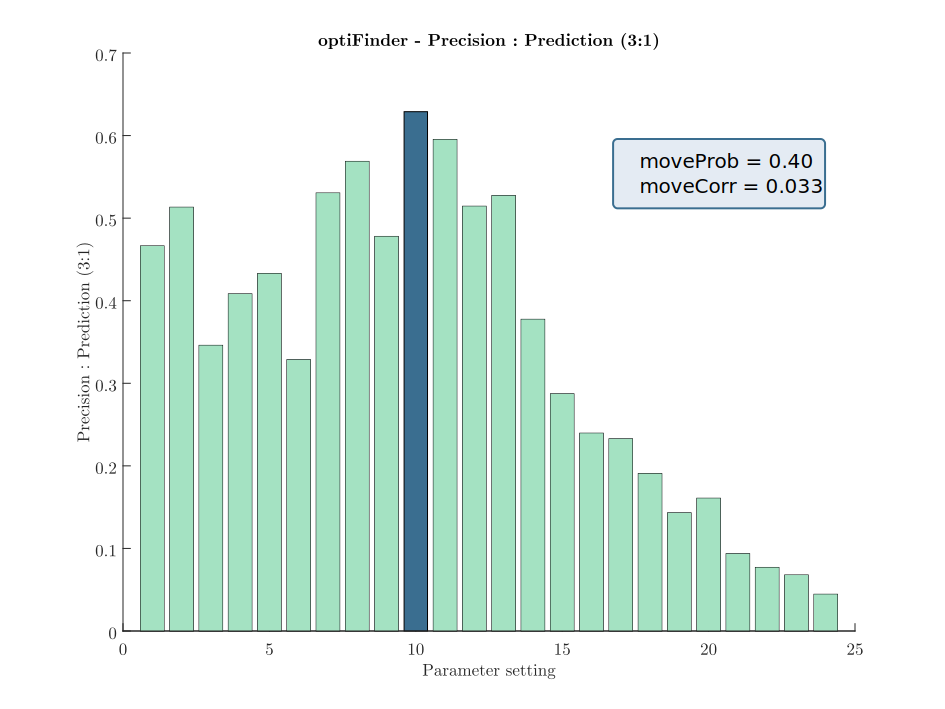
\includegraphics[width=\textwidth]{prepred1.pdf}
\end{minipage}
\begin{minipage}[t]{.48\textwidth}
\includegraphics[width=\textwidth]{prepred2.pdf}
\end{minipage}
\caption{left: Dataset 1, right: Dataset 2, values from prediction (1x) and precision (3x)}
\end{figure}

The mean of the two found parameters are: \\$moveProb = 0.425$ and $moveCorr = 0.066$.

\begin{figure}[H]
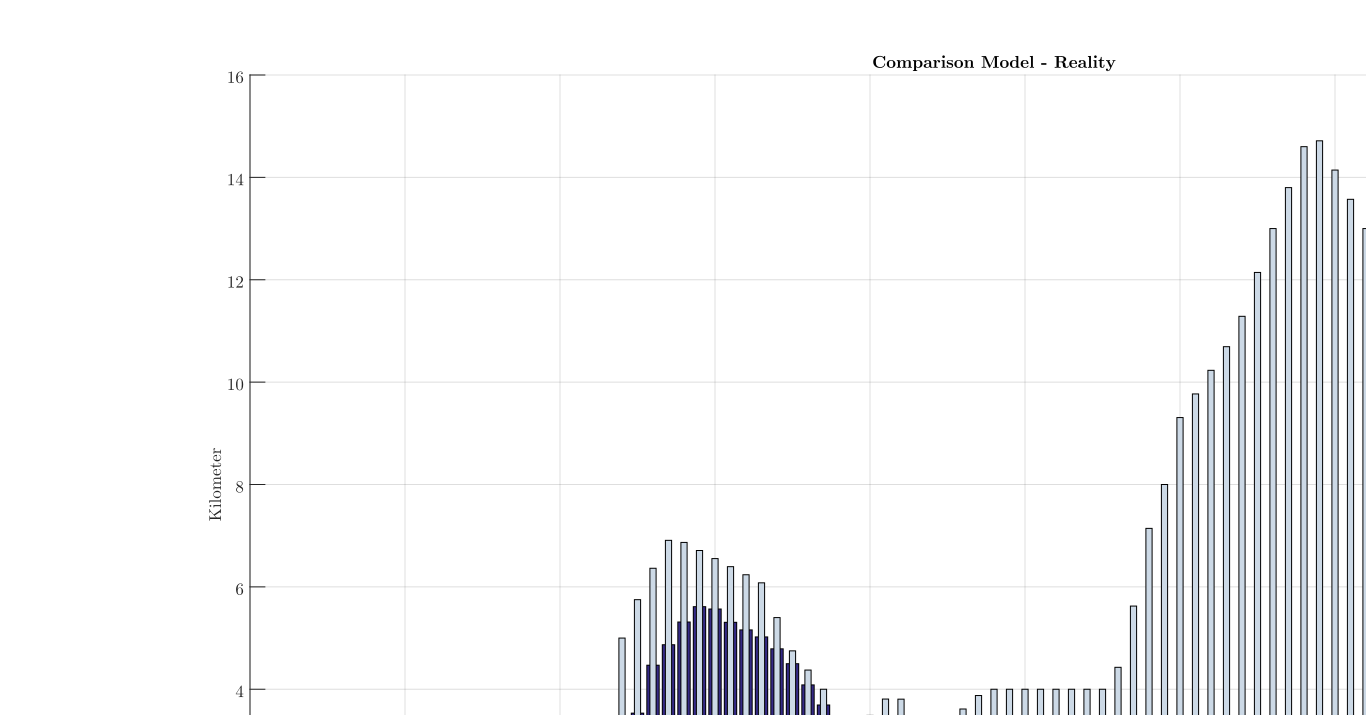
\includegraphics[width=\textwidth]{dataset3.pdf}
\caption{Dataset 3 --  precision = 0.31, prediction = 0.84}
\end{figure}

\begin{figure}[H]
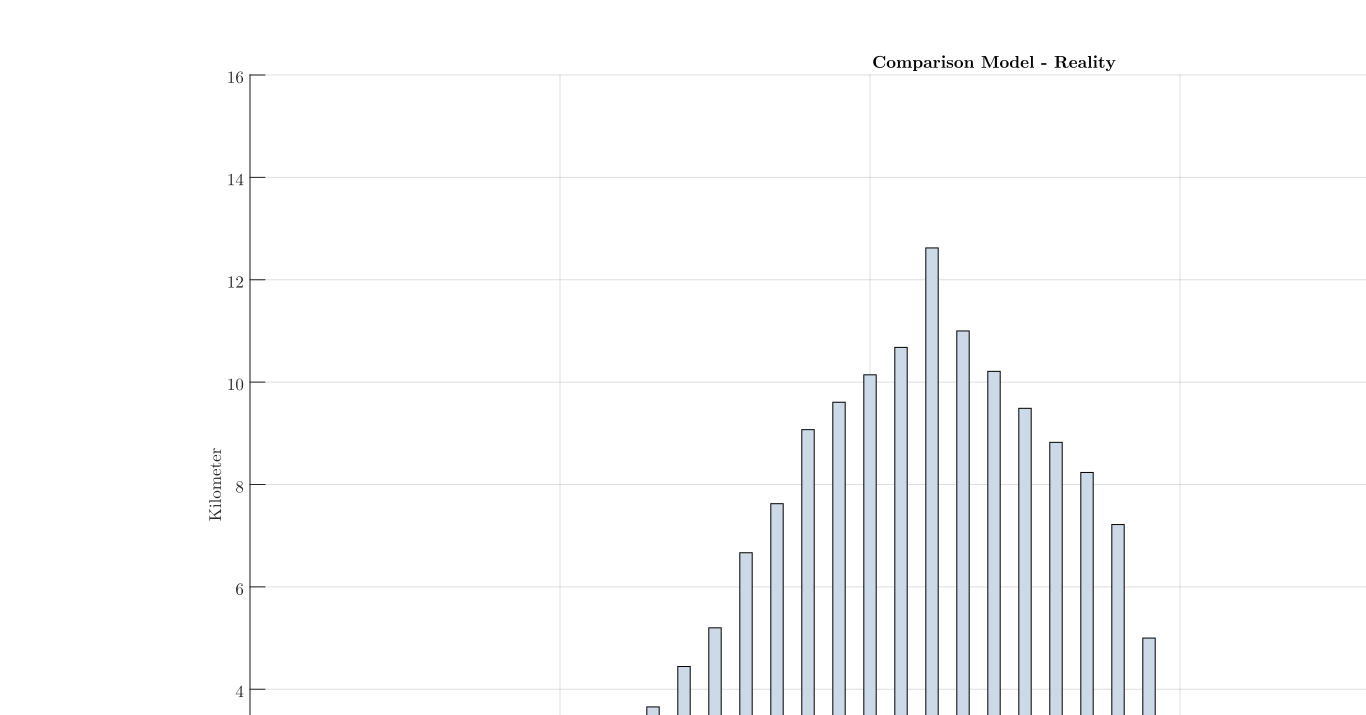
\includegraphics[width=\textwidth]{dataset4.pdf}
\caption{Dataset 4 --  precision = 0.17, prediction = 0.77}
\end{figure}
